\documentclass{article}
\usepackage[utf8]{inputenc}
\usepackage{amsmath}
\usepackage{amssymb}
\usepackage{graphicx}
\usepackage{geometry}
\geometry{a4paper, margin=1in}

\title{CSCI-UA.0480-051: Parallel Computing Midterm Exam (Mar 14th, 2024)}
\author{Your Name}
\date{March 14th, 2024}

\begin{document}

\maketitle

\textbf{Total: 100 points}

\textbf{Important Notes - READ BEFORE SOLVING THE EXAM}

\begin{itemize}
    \item If you perceive any ambiguity in any of the questions, state your assumptions clearly and solve the problem based on your assumptions. We will grade both your solutions and your assumptions.
    \item This exam is take-home.
    \item The exam is posted on Brightspace, at the beginning of the March 14th lecture (2pm EST).
    \item You have up to 24 hours to submit on Brightspace (i.e. till March 15th 2pm EST), in the same way as you submit an assignment. However, unlike assignments, you can only submit once.
    \item Your answers must be very focused. You may be penalized for giving wrong answers and for putting irrelevant information in your answers.
    \item Your answer sheet must be organized as follows:
    \begin{itemize}
        \item The very first page of your answer must contain only:
        \begin{itemize}
            \item Your Last Name
            \item Your First Name
            \item Your NetID
            \item Copy and paste the honor code shown below.
        \end{itemize}
        \item In your answer sheet, answer one problem per page. The exam has seven main problems, each one must be answered in a separate page.
    \end{itemize}
    \item This exam consists of 7 problems, with a total of 100 points.
    \item Your answers can be typed or written by hand (but with clear handwriting). It is up to you. But you must upload one pdf file containing all your answers.
\end{itemize}

\textbf{Honor code (copy and paste to the first page of your exam)}
\begin{itemize}
    \item You may use the textbook, slides, the class recorded lectures, the information in the discussion forums of the class on Brightspace, and any notes you have. But you may not use the internet.
    \item You may NOT use communication tools to collaborate with other humans. This includes but is not limited to Google-Chat, Messenger, E-mail, etc.
    \item You cannot use LLMs such as chatGPT, Gemini, Bard, etc.
    \item Do not try to search for answers on the internet, it will show in your answer, and you will earn an immediate grade of 0.
    \item Anyone found sharing answers, communicating with another student, searching the internet, or using prohibited tools (as mentioned above) during the exam period will earn an immediate grade of 0.
    \item “I understand the ground rules and agree to abide by them. I will not share answers or assist another student during this exam, nor will I seek assistance from another student or attempt to view their answers.”
\end{itemize}


\section*{Problem 1}
\begin{enumerate}
    \item[a.] [10] Explain Amdahl's Law in the context of parallel computing.  Give a specific example of a computation where Amdahl's Law would significantly limit speedup.
    \item[b.] [10] What are the main differences between OpenMP and MPI?  Discuss their strengths and weaknesses in different parallel computing scenarios.
    \item[c.] [10] Describe the concept of a race condition in parallel programming. Provide a simple code snippet (in C or pseudocode) illustrating a race condition and explain how it can be avoided.
    \item[d.] [6]  What is the purpose of a barrier synchronization in parallel programming? Explain a situation where a barrier is crucial for correctness.
\end{enumerate}

\section*{Problem 2}
Consider the following DAG representing a parallel computation:

\begin{center}
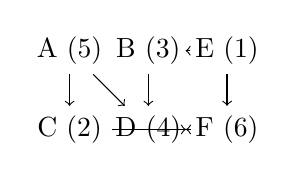
\begin{tikzpicture}[node distance=1cm]
\node (A) {A (5)};
\node (B) [right of=A] {B (3)};
\node (C) [below of=A] {C (2)};
\node (D) [below of=B] {D (4)};
\node (E) [right of=B] {E (1)};
\node (F) [right of=D] {F (6)};
\draw[->] (A) -- (C);
\draw[->] (A) -- (D);
\draw[->] (B) -- (D);
\draw[->] (B) -- (E);
\draw[->] (C) -- (F);
\draw[->] (D) -- (F);
\draw[->] (E) -- (F);
\end{tikzpicture}
\end{center}

Numbers in parentheses represent the execution time of each task in milliseconds.

\begin{enumerate}
    \item[a.] [10]  Determine the critical path of this DAG and calculate the minimum execution time for the entire computation.
    \item[b.] [10]  Suppose we have two identical CPUs. Schedule the tasks to minimize the overall execution time. Show your schedule and calculate the speedup compared to sequential execution.
    \item[c.] [10] If we have three CPUs, how would you schedule the tasks? Show your schedule and calculate the speedup.
\end{enumerate}

\section*{Problem 3}
The following code uses MPI to compute the sum of an array distributed among multiple processes.

\begin{verbatim}
#include <mpi.h>
#include <stdio.h>

int main(int argc, char** argv) {
    int rank, size;
    int n = 10;
    int local_sum = 0;
    int global_sum = 0;
    int data[10] = {1, 2, 3, 4, 5, 6, 7, 8, 9, 10};

    MPI_Init(&argc, &argv);
    MPI_Comm_rank(MPI_COMM_WORLD, &rank);
    MPI_Comm_size(MPI_COMM_WORLD, &size);

    //Local sum calculation
    for (int i = rank * (n / size); i < (rank + 1) * (n / size); i++) {
        local_sum += data[i];
    }

    //Reduce to global sum
    MPI_Reduce(&local_sum, &global_sum, 1, MPI_INT, MPI_SUM, 0, MPI_COMM_WORLD);

    if (rank == 0) {
        printf("Global sum: %d\n", global_sum);
    }

    MPI_Finalize();
    return 0;
}
\end{verbatim}

\begin{enumerate}
    \item[a.] [8]  Explain what will happen if you run this code with 4 processes. Show the values of `local_sum` and `global_sum` for each process.
    \item[b.] [7]  What will happen if `n` is not a multiple of `size`? Modify the code to handle this case correctly.
    \item[c.] [10]  Assume you have a very large array that doesn't fit in a single process's memory. How would you modify the code to handle this situation?  Explain your approach and potential challenges.

\end{enumerate}


\section*{Problem 4}
\begin{enumerate}
    \item[a.] [10] Describe the concept of false sharing in shared-memory programming.  Give an example and explain how it can be mitigated.
    \item[b.] [10]  Compare and contrast the performance characteristics of different types of cache coherency protocols (e.g., write-invalidate, write-update).
\end{enumerate}

\section*{Problem 5}
Consider a parallel algorithm that sorts a large array using a divide-and-conquer approach. The array is divided into multiple sub-arrays, each sorted independently by a different processor. Then a merging phase combines the sorted sub-arrays.

\begin{enumerate}
    \item[a.] [10] Describe a suitable parallel sorting algorithm for this problem.
    \item[b.] [10] Discuss the scalability of this algorithm.  How does the performance scale with the number of processors and the size of the input array?  What are the limiting factors?
\end{enumerate}

\section*{Problem 6}
\begin{enumerate}
    \item[a.] [12] Explain the difference between strong and weak scaling in parallel computing.  Provide examples of applications that are likely to exhibit strong scaling and those that are more likely to exhibit weak scaling.
    \item[b.] [8] What are some common performance bottlenecks in parallel programs? How can you identify and address these bottlenecks?
\end{enumerate}

\section*{Problem 7}
\begin{enumerate}
    \item[a.] [10] Describe the concept of a deadlock in parallel programming. Provide a simple scenario (using pseudocode or a diagram) that could lead to a deadlock.
    \item[b.] [10] Explain different techniques for preventing or detecting deadlocks in parallel programs.
\end{enumerate}

\end{document}